\documentclass[11pt,fleqn]{exam}
\usepackage[utf8]{inputenc}
\usepackage[T1]{fontenc}
\usepackage{fancyvrb}
\usepackage{amsmath}
\usepackage{amssymb}
\usepackage{hyperref}
\usepackage{algpseudocode}
\usepackage{algorithm,algorithmicx}
\usepackage{comment}
\usepackage{enumitem}
\usepackage[margin=0.75in]{geometry}
\usepackage{tikz}
\usetikzlibrary{arrows,arrows.meta,positioning,intersections,shapes.gates.logic.US,calc,trees}
\algnewcommand\algorithmicforeach{\textbf{for each}}
\algdef{S}[FOR]{ForEach}[1]{\algorithmicforeach\ #1\ \algorithmicdo}
\newcommand{\fillinMCmath}[1]{
\begin{tikzpicture}\draw circle [radius=0.5em];\end{tikzpicture}\ #1}
\newcommand{\fillinMCmathsoln}[1]{
\begin{tikzpicture}\draw[black, fill=blue] circle [radius=0.5em];\end{tikzpicture}\ #1}
\newcommand{\fillinblank}[1]{\fillinblankmath{\mbox{#1}}}
\newcommand{\fillinblankmath}[1]{\begingroup\setlength{\fboxsep}{1em}\setlength{\fboxrule}
{2pt}\fbox{\LARGE\phantom{#1}}\endgroup}
\newcommand{\fillinblankmathsoln}[1]{\begingroup\setlength{\fboxsep}{1em}\setlength{\fboxrule}
{2pt}\fbox{#1}\endgroup}
\newcommand{\ptsamt}[1]{[#1~points]}
\newcommand{\ptamt}[1]{[#1~point]}

%%% Adding Colour to Questions and Answers
\usepackage{color}

\definecolor{solnblue}{rgb}{0,0,1}
\newenvironment{soln}{\color{solnblue}}{}

%fancyvrb commands
\def\lar{$\leftarrow$}
\def\lesseq{$\leq$}
\def\greq{$\geq$}
\def\alp{$\alpha$}
\def\inf{$\infty$}
\def\ne{$\neq$}

\newcommand{\subsum}{\mbox{SS}}
\newcommand{\sub}{\mbox{Sub}}

%Questions

% Answers
\definecolor{blu}{rgb}{0,0,0.5}
\def\blu#1{{\color{blu}#1}}
\definecolor{gre}{rgb}{0,.3,0}
\def\gre#1{{\color{gre}#1}}
\definecolor{red}{rgb}{0.5,0.0,0}
\def\red#1{{\color{red}#1}}
\def\norm#1{\|#1\|}
%%% End for Colours

\bracketedpoints


\makeatletter
\renewenvironment{solution}{\leavevmode\par\begin{soln}\noindent Solution:}{\end{soln}}
\makeatother
 \newif\ifsolutions\solutionstrue
 
\author{}
\date{}

% \newif\ifsolutions\solutionstrue
\newif\ifsolutions\solutionsfalse

\ifsolutions
\title{COSC 320: Assignment 4 Solutions}
\else
\title{COSC 320: Assignment 4}
\fi

\begin{document}

	\maketitle
	
	
	\ifsolutions
\setcounter{section}{2}
\else
This assignment is due \textbf{Friday, March 14 at 7 PM}. Late submissions will not be accepted. All the submission and formatting rules for Assignment~1 apply to this assignment as well.  

%------------------------------------------------------------------------------------
\section{List of names of group members (as listed on Canvas)}

Provide the list here. This is worth 1 mark. Include student numbers as a secondary failsafe if you wish.

\begin{enumerate}
   \item Rin Meng, 51940633
   \item Mika Panagsagan 29679552
    \item Kevin Zhang 10811057
\end{enumerate}

\section{Statement on collaboration and use of resources}
To develop good practices in doing homeworks, citing resources and acknowledging input from others, please complete the following. This question is worth 2 marks.

\begin{enumerate}
\item All group members have read and followed the guidelines for groupwork on assignments given in the Syllabus).

\fillinMCmathsoln{Yes} \hspace{.5in} \fillinMCmath{No}

\item We used the following resources (list books, online sources, etc. that you consulted):
\begin{soln}
   \begin{enumerate}
       \item DeepSeek R1, ChatGPT to generate ideas, explain concepts, and check if we are going in the right direction.
       \item Google Search, Google's AI Overview
       \item COSC 320 Lecture Slides
    \end{enumerate}
\end{soln}

\item One or more of us consulted with course staff during office hours.

\fillinMCmath{Yes} \hspace{.5in} \fillinMCmathsoln{No}

\item One or more of us collaborated with other COSC 320 students; none of us took
      written notes during our consultations and we took at least a half-hour break afterwards.

\fillinMCmath{Yes} \hspace{.5in} \fillinMCmathsoln{No}

      If yes, please list their name(s) here:

\item One or more of us collaborated with or consulted others outside of COSC 320; none of us took written notes during our consultations and we took at least a half-hour break afterwards.

\fillinMCmath{Yes} \hspace{.5in} \fillinMCmathsoln{No}

      If yes, please list their name(s) here:

\end{enumerate}
\newpage
\fi

%==========================================
	
	\section{Mystery QuickSelect}
The following variant of the QuickSelect algorithm carefully chooses a pivot, so as to
guarantee that the sizes of Lesser and Greater are at most $7n/10$, and may equal $7n/10$ in the worst case.
It does this by choosing $\lceil n/5 \rceil$ elements in $\Theta(n)$ time (line 7 below), and setting the
pivot to be the median of these elements via a recursive call (line 8).
Exactly how the $\lceil n/5 \rceil$ elements are chosen is not
important.  The rest of the algorithm is identical to \textsc{QuickSelect}.

\vspace{.1in}

\begin{algorithmic}[1]
\Function{MysteryQuickSelect}{$A[1..n], k$}
\State $\triangleright$ return the $k$th smallest element of $A$, where $1\le k \le n$ and all elements of $A$ are distinct
\If{$n==1$}
   \State \Return $A[1]$
\Else
   \State $\triangleright$ the next two lines select the pivot element $p$
   \State create array $A'$ of $\lceil n/5 \rceil$ "carefully choosen" elements of $A$ \Comment this takes $\Theta(n)$ time
    \State $p \gets$ \textsc{MysteryQuickSelect}($A', \lceil |A'|/2 \rceil$) \Comment $A'$ has  $\lceil n/5\rceil$ elements
    \State Lesser  $\gets$ all elements from $A$ less than $p$  \Comment Lesser has $7n/10$ elements in the worst case
    \State Greater $\gets$ all elements from $A$ greater than $p$ \Comment Greater has $7n/10$ elements in the worst case

    \If{|Lessor| $\ge k$}
       \State \Return \textsc{MysteryQuickSelect}(Lesser, $k$)
    \ElsIf{|Lesser| $ = k - 1$}
        \State \Return $p$
   \Else  \hspace{.2in} $\triangleright$ |Lesser| $< k-1$
       \State \Return \textsc{MysteryQuickSelect}(Greater, $k - |\mbox{Lesser}| - 1$)
   \EndIf
\EndIf
\EndFunction
\end{algorithmic}

\begin{questions}
\question[3]
Let $T'(n)$ be the {\em worst-case} run time of \textsc{MysteryQuickSelect}. Complete the following
recurrence for $T'(n)$. by replacing the parts with ???s. You can ignore floors and ceilings.  No justification needed.
%Use the facts that the pivot partitions a problem of size $n$ into subproblems of size at most $7n/10$ and that
%the time to create list $A'$ is $O(n)$.

\ifsolutions
\input{q3a-soln.tex}
\clearpage
   \else
 \[
   T'(n) = \left\{ \begin{array}{ll}
               c, & \mbox{ if }  \mbox{???} \\
            \mbox{ ???} + cn , & \mbox{ if } n > 1
             \end{array} \right.
   \]

\fi


\begin{soln}
   \[
   T'(n) = \left\{ \begin{array}{ll}
               c, & \mbox{ if }  n = 1 \\
            T^\prime(\frac{n}{5}) + T^\prime(\frac{7n}{10}) + cn , & \mbox{ if } n > 1
             \end{array} \right.
   \]
\end{soln}

\question[3]
Draw the first three levels (0,1, and 2) of the recursion tree for your recurrence. Label each node with the size of the subproblem it represents, as well as the work done at that node not counting recursive calls. Finally, put the total work per level in a column on the right hand side of your tree. You can provide a hand-drawn figure as long as it is clear and legible. 

\ifsolutions
\vspace{.1in}
\input{q3b-soln.tex}
\else
\fi

\begin{soln}
   \begin{center}
      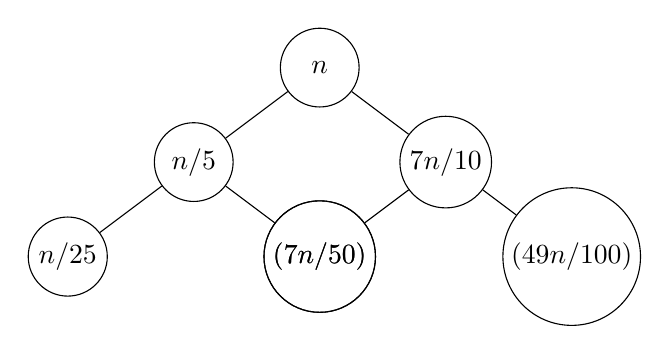
\begin{tikzpicture}[scale=0.8, level distance=1.5cm, sibling distance=4cm,
        every node/.style={draw, circle, minimum size=1cm, inner sep=2pt}]
        
        \node {$n$}
          child { node {$n/5$}
            child { node {$n/25$} }
            child { node {$(7n/50)$} }
          }
          child { node {$7n/10$}
            child { node {$(7n/50)$} }
            child { node {$(49n/100)$} }
          };
      \end{tikzpicture}
      \end{center}
      
      \begin{center}
      \begin{tabular}{cc}
        Level & Total Work Per Level \\
        \hline
        0 & $O(n)$ \\
        1 & $O(n/5) + O(7n/10) = O(n)$ \\
        2 & $O(n/25) + O(7n/50) + O(7n/50) + O(49n/100) = O(n)$
      \end{tabular}
      \end{center}
\end{soln}

\vspace{.1in}

\question[2]
What is the worst-case runtime of \textsc{MysteryQuickSelect}? Provide a short justification of your answer.

\begin{soln}
   The worst-case runtime of \textsc{MysteryQuickSelect} is $O(n)$. 
   This is because the recurrence $T'(n) = T'(n/5) + T'(7n/10) + cn$ gets solved to $O(n)$,
   as shown in the previous question.
\end{soln}

\ifsolutions
 \input{q3c-soln.tex}
 \else
 \fi
\question[2]
For comparison, what is the worst case runtime of the {\em original}  \textsc{QuickSelect} algorithm from the worksheet, in which lines 7 and 8 of the pseudocode above are replaced by setting the pivot $p$ to $A[1]$?  Provide a short justification of your answer.

\begin{soln}
   Line 8 of the pseudocode above is replaced by setting the pivot $p$ to
    $A[1]$, which results in the worst-case runtime of $O(n^2)$.
   \begin{itemize}
      \item In the worst case, every recursive call only removes one element from the list, so the 
      recurrence is $T(n) = T(n-1) + cn$.
      \item This results to a linear depth recursion tree, and the total work done is $O(n^2)$.
      \item This is similar to the worst case of QuickSort.
   \end{itemize}
\end{soln}


\ifsolutions
\input{q3d-soln.tex}
\else
\fi

\end{questions}

\newpage
	        
\section{Subway Sub-array}

[Thanks to Peter Gu for contributing this problem.]

\vspace{.1in}

\noindent
Peter has just purchased a sandwich from the Life Building Subway. The sandwich can be represented as an array $A$ of $n$ real-valued quantities. Peter is peculiar, he enjoys partitioning his sandwich into contiguous sub-arrays such that every element from the original array belongs to a sub-array. He then scores each sub-array $A[l,r], 1 \le l \le r \le n$ with the following formula:
\[
    \subsum(l,r) = ax^2 + bx + c,
\]
where $a, b, c \in \mathbb{Z}$ and $x$ is the sum of all elements in the sub-array $A[l..r]$. He would like you to develop an algorithm to find the score of a partition that maximizes the sum of the scores of its subarrays.

More formally, an instance of the problem consists of the array $A[1..n]$ plus the quantities $a, b$, and $c$, and the goal is to determine $\sub(n)$, defined as follows when $n \ge 1$:
\[
\sub(n) = \max_{1\le k \le n}  \;\; \max_{0 = p_0 < p_1 < p_2 < \ldots < p_k = n} \;\; \subsum(p_0+1,p_1) + \subsum(p_1+1,p_2) +  \subsum(p_2+1,p_3) + \ldots \subsum(p_{k-1}+1,p_k).
\]
(Here, $k$ is the number of subarrays in the partition, and for $1 \le i \le k$, the $i$th subarray ranges from $p_{i-1}+1$ to $p_i$.) We'll also define $\sub(0)$ to be 0.
\vspace{.1in}

\noindent
{\bf Example:} Suppose that the array is $[1, 2, -3, 2, 1]$ and $a = 1, b = 1, c = 5$. One possible partition into subarrays is $[1, 2], [-3], [2, 1]$. The respective scores for this partition are $[3^2 + 3 + 5], [3^2 - 3 + 5], [3^2 + 3 + 5]$ and the total sum is $45$. 

Note: No justification is needed for the first five parts of this problem.

\begin{questions}
\question[1]
For the example array above, give an optimal partition and write down its value $\sub(5)$.

\begin{soln}
   One possible optimal partition is $[1, 2], [-3], [2, 1]$, with a total score of $45$ which
   was given in the example.
\end{soln}

\ifsolutions
\input{q4aa-soln.tex}
\else
\fi

\question[3]
Provide pseudocode to calculate all of the quantities $\subsum(l,r)$, for $1\le l \le r \le n$. 
Your pseudocode should run in $O(n^2)$ time.

\begin{soln}
   \begin{algorithmic}[1]
      \Function{CalculateAllQuanitites}{$A[1..n], a, b, c$}
         \State $n \gets \mbox{length}(A)$
         \State $Q[1..n][1..n] \gets 0$
         \For{$l = 1$ to $n$}
            \For{$r = l$ to $n$}
               \State $x \gets 0$
               \For{$i = l$ to $r$}
                  \State $x \gets x + A[i]$
               \EndFor
               \State $Q[l][r] \gets a \cdot x^2 + b \cdot x + c$
            \EndFor
         \EndFor
         \State \Return $Q$
      \EndFunction
   \end{algorithmic}
\end{soln}


\ifsolutions
\input{q4a-soln.tex}
\else
\fi

\question[3]
Let $n \ge 1$.
Suppose that in an optimal partition, the rightmost subarray is $A[i+1..n]$, where $0 \le i \le n-1$. Write down an expression for the value of $\sub(n)$  in terms of the quantity $\subsum(i+1,n)$ and the function $\sub()$ applied to a smaller problem instance.

\begin{soln}
   For $n \geq 1$, $A[i+1..n]$, $0 \le i \le n-1$, $SS(i+1,n)$ 
   \[
   \sub(n) = \max_{0 \le i \le n-1} \left( \subsum(i+1,n) + \sub(i) \right)
   \]
\end{soln}


\ifsolutions
\input{q4b-soln.tex}
\else
\fi

\question[2]
Provide a recurrence for $\sub(n)$. Your answer to the previous part should be useful.

\begin{soln}
   Base case $n = 0$: $\sub(0) = 0$.
   For $n \geq 1$, $\sub(n) = \max_{0 \le i \le n-1} \left( \subsum(i+1,n) + \sub(i) \right)$.
   Therefore the recurrence is:
   \[
   \sub(n) = \left\{ \begin{array}{ll}
               0, & \mbox{ if } n = 0 \\
            \max_{0 \le i \le n-1} \left( \subsum(i+1,n) + \sub(i) \right), & \mbox{ if } n > 0
             \end{array} \right.
   \]

\end{soln}

\ifsolutions
\input{q4c-soln.tex}
\else
\fi

\question[5]
Using the recurrence, develop a memoized algorithm to compute $\sub(n)$. Remember that a memoized algorithm is always recursive. Your algorithm can use the quantities $\subsum(l,r)$ (since these values can be pre-computed by your algorithm from part 1 above).

\begin{soln}
   \begin{algorithmic}[1]
      \Function{MemoizedSub}{$A[1..n], a, b, c$}
         \State $n \gets \mbox{length}(A)$
         \State $Q \gets \mbox{CalculateAllQuantities}(A, a, b, c)$
         \State $M[0..n] \gets \mbox{None}$ 
         \State \Return $\mbox{MemoizedSubHelper}(A, a, b, c, Q, n, M)$
      \EndFunction
      \State
      \Function{MemoizedSubHelper}{$A[1..n], a, b, c, Q, n, M$}
         \If{$n == 0$}
            \State \Return 0
         \EndIf
         \If{$M[n] \neq \mbox{None}$}
            \State \Return $M[n]$
         \EndIf
         \State $M[n] \gets -\infty$  \Comment{Set to smallest possible value}
         \For{$i = 0$ to $n-1$}
            \State $M[n] \gets \max(M[n], Q[i+1][n] + \mbox{MemoizedSubHelper}(A, a, b, c, Q, i, M))$
         \EndFor
         \State \Return $M[n]$
      \EndFunction
\end{algorithmic}

\end{soln}


\ifsolutions
\input{q4d-soln.tex}
\else
\fi


\question[2]
What is the runtime of your memoized algorithm?  Provide a short justification.

\begin{soln}
   The runtime of the memoized algorithm is $O(n^2)$.
   \begin{itemize}
      \item The algorithm computes all the quantities $\subsum(l,r)$ in $O(n^2)$ time.
      \item The memoized algorithm computes $\sub(n)$ using the recurrence in $O(n)$ time.
      \item The total runtime is $O(n^2)$.
   \end{itemize}
\end{soln}

\ifsolutions
\input{q4e-soln.tex}
\else
\fi

\question[3]
Bonus: Suppose that instead of using the $\subsum()$ function to score a subarray, now use a linear variant:
\[
    \subsum'(l,r) = bx + c,
\]
where $b, c \in \mathbb{Z}$ and $x$ is the sum of all the elements in the sub-array $A[l..r]$. For this variant, we want to find the score of a partition that maximizes the sum of all subarrays.  Explain how we can achieve this with an algorithm whose runtime is faster than that for the original problem.

\ifsolutions
\input{q4f-soln.tex}
\else
\fi

\end{questions}

\newpage

%=========================================================================================
\section{Legend of Zelda}

[Thanks to Denis Lalaj for contributing this problem.]

\vspace{.1in}

An instance of the problem is $G[1..m][1..n]$---a 2D array of size $m \times n$ where each entry $G[i,j]$ is an integer (either positive or negative), representing the points  that Link can accumulate in the room at coordinates $(i,j)$. 

Link starts his quest at room $(1,1)$ and needs to get to the $(m,n)$ corner, via a path where each move is either to the right or downwards. Link starts with some initial number of points, and upon entering each room (including the first), Link's points are adjusted up or down by adding the points in that room. Link must ensure that he always has at least one point.

For $1 \le i \le m$ and $1\le j \le m$, let $HP[i,j]$ denote the minimum number of points that Link needs to have, when starting by entering the room with coordinates $(i, j)$, in order to reach $(m,n)$ while always having at least one point. The problem is to compute $HP[1,1]$---the minimum number of points needed initially in the full game.

We have the following recurrence for $HP[i,j]$:

\[
HP[i,j] = \left\{\begin{array}{ll}
\max(1, 1-G[m,n]), & \mbox{ if  $i=m$ and  $j=n$},\\
\max(1, \min(HP[i+1,j], HP[i,j+1]) -  G[i,j]), & \mbox{ if $1 \le i \le m-1$ or $1\le j \le n-1$}, \\
\infty,  & \mbox{ if $i = m+1$ or $j = n+1$}.
\end{array}
\right.
\]

\begin{questions}
\question[5]
Using this recurrence, 
develop a dynamic programming algorithm  to compute $HP(1,1)$. Remember that a dynamic programming algorithm is iterative (involving loops), not recursive.

\begin{soln}
   \begin{algorithmic}[1]
      \Function{HP}{$G[1..m][1..n]$}
         \State $m \gets \text{# rows of } G$
         \State $n \gets \text{# columns of } G$
         \State $HP[m+1][n+1] \gets \infty$
         \State $HP[m][n] \gets \max(1, 1 - G[m,n])$
         \For{$i = m$ down to $1$}
            \For{$j = n$ down to $1$}
               \If{$i == m$ and $j == n$}
               \State $\min HP \gets \min(HP[i+1,j], HP[i,j+1])$
               \State $HP[i,j] \gets \max(HP[i+1,j], HP[i,j+1]) - G[i,j]$
               \EndIf
            \EndFor
         \EndFor
         \State \Return $HP[1,1]$
      \EndFunction
   \end{algorithmic}
\end{soln}


\ifsolutions
\input{q5a-soln.tex}
\else
\fi

\question[2]
What is the runtime of each of your algorithm?  Provide a short justification.

\begin{soln}
   The runtime of the dynamic programming algorithm is $O(mn)$.
   \begin{itemize}
      \item It's a double loop that iterates over all the rooms in the grid, so the runtime is $O(mn)$.
      \item It is a 2D array of size $m \times n$.
   \end{itemize}
\end{soln}

\ifsolutions
\input{q5b-soln.tex}
\else
\fi

\question[Optional: 0]
 Use the recurrence above to write a memoized algorithm to compute $HP(1,1)$.
\end{questions}


\end{document}